% 96-34(96쪽) — 연속함수 f(x)의 도함수 y=f'(x) 의 그래프(왼쪽 내리막 직선 + x>=1 에서 수평선 y=2). 스캔 화질이 낮아 TikZ 로 다시 그림.
% 원문에 있는 것만: 눈금 숫자 4 · 2 (y) · 1 (x) · 라벨 O, x, y, y=f'(x) · (0,2)-(1,2) 와 (1,0)-(1,2) 안내 파선.
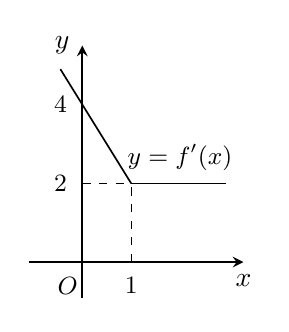
\begin{tikzpicture}[x=0.62cm, y=0.50cm, line width=0.5pt]
  \draw[->, >=stealth, line width=0.7pt] (-1.1,0) -- (3.3,0) node[below=1pt] {$x$};
  \draw[->, >=stealth, line width=0.7pt] (0,-0.9) -- (0,5.5) node[left=1pt] {$y$};
  \node[below=2pt, font=\small] at (-0.3,0) {$\pt{O}$};
  % 좌표 안내 파선(원문)
  \draw[dashed, line width=0.35pt] (0,2) -- (1,2);
  \draw[dashed, line width=0.35pt] (1,0) -- (1,2);
  % 그래프
  \draw[line width=0.6pt] (-0.45,4.9) -- (1,2);
  \draw[line width=0.6pt] (1,2) -- (2.95,2);
  % 눈금 라벨(원문 자리 그대로)
  \node[left=2pt, font=\small] at (0,4) {$4$};
  \node[left=2pt, font=\small] at (0,2) {$2$};
  \node[below=2pt, font=\small] at (1,0) {$1$};
  \node[above=1pt, font=\small] at (2.0,2) {$y=f'(x)$};
\end{tikzpicture}
